%\documentclass[useAMS,usenatbib,useAMS,referee]{mn2e}
\documentclass[useAMS,usenatbib]{mn2e}
\usepackage{times}
\usepackage{graphicx}
%\usepackage{amsmath}
%\usepackage{amssymb}
\usepackage{latexsym}
\usepackage{subfigure}

%%%%% AUTHORS - PLACE YOUR OWN MACROS HERE %%%%%
%%%%%%%%%%%%%%%%%%%%%%%%%%%%%%%%%%%%%%%%%%%%%%%%
\newcommand{\mnras}{MNRAS}
\newcommand{\apj}{ApJ}
\newcommand{\aap}{A\&A}

\title[On the validity of the Perturbative Approach for Strong Gravitational Lensing]{On the validity of the Perturbative Approach for Strong Gravitational Lensing: Local Distortion for Pseudo-Elliptical Models}
\author[H.S.~D\'umet-Montoya et. al.]{H. S. D\'umet-Montoya$^{1}$\thanks{E-mail:
habibdumet@gmail.com ; hdumetm@cbpf.br }, G.~B. Caminha$^{1}$, B.~Moraes$^{1}$, M. Makler$^{1}$ and 
Mandeep Gill$^{2}$\\
$^{1}$Centro Brasileiro de Pesquisas F\'isicas, Rio de Janeiro\\
$^{2}$Ohio State Univ, United States}
% and DES-Brazil builders.


\begin{document}

\date{Accepted: Algum dia }

\pagerange{\pageref{firstpage}--\pageref{lastpage}} \pubyear{2011}

\maketitle

\label{firstpage}

\begin{abstract}
We investigated the validity of the Perturbative Approach for Strong Gravitational Lensing, which was proposed by Alard on
basis of a solution around the Einstein Radius. We adopt Pseudo-Elliptical models, such SIEP and PNFW
\end{abstract}

\begin{keywords}
galaxies:cluster:general, cosmology: dark matter, gravitational lensing: strong.
\end{keywords}

\section{Introduction}

The introduction must be contain
\begin{itemize}
\item Motivation for Gravitational Arcs
\item Potentially application of the Perturbative Approach
\item Motivation for Pseudo-Elliptical Models
\item Motivation for the Cross Section
\end{itemize}

\section{Basics of Gravitational Lensing}

\subsection{General Lensing Equations}

In this section, we define the lensing functions as well as equations and useful relations that will be needed later on.  In this work, we assume the thin-screen approximation and that the lens and source are centered in their corresponding planes.

We refer to $\bmath{\xi}$ and $\bmath{\eta}$ as the physical coordinates of the lens and the source planes respectively. We use the characteristic scales  $\xi_0$ in the lens plane, and $\eta_0= \xi_0 D_{\rm OL}/D_{\rm OS}$ in the source plane, where $D_{\rm OS}$ is the angular diameter distance between source and observer, $D_{\rm OL}$ is the distance between lens and observer. Also, $D_{\rm LS}$ is defined as the distance between the lens and source. These scales allow us to write the main lensing quantities as a function of dimensionless coordinates $\bmath{x}=\bmath{\xi}/\xi_0$ in the lens plane and $ \bmath{y}=\bmath{\eta}/\eta_0$ in the source plane.

The position of a source and its corresponding image (or images) are related by the lens equation \citep{SEF}
\begin{equation}
\bmath{y}=\bmath{x}-\bmath{\alpha}(\bmath{x})
\label{lens_eq_ad}
\end{equation}
where $\bmath{\alpha}$ is the reduced deflection angle at position $\bmath{x}$, and is given by the gradient of the 2D lensing potential $\varphi(\bmath{x})$
\begin{equation}
\bmath{\alpha}(\bmath{x})=\nabla_{\bmath{x}}\varphi(\bmath{x}) \label{angled_ex1},
\end{equation}
or by the sum of the deflections due to all the mass elements in the plane
\begin{equation}
\bmath{\alpha}(\bmath{x})=\frac{1}{x}\int d^2x^\prime \frac{\Sigma(\xi_0\bmath{x})}{\Sigma_{\rm crit}}\frac{\bmath{x}-\bmath{x}^\prime}{|\bmath{x}-\bmath{x}^\prime|} \label{angled_ex2},
\end{equation}
where
\[
\Sigma_{\rm crit}=\frac{c^2 D_{\rm OS}}{4\pi G D_{\rm LS}D_{\rm OL}}
\]
is the critical surface mass density, a quantity which characterizes the lens system.

The lensing functions as the convergence and components of the shear can be derived from the deflexion angle
%\begin{eqnarray}
%\kappa(\bmath{x})&=&\frac{1}{2}\left(\partial_1 \alpha_1+ \partial_2 \alpha_2\right) \nonumber \\
%\gamma_1(\bmath{x})&=& \frac{1}{2}\left(\partial_1 \alpha_1- \partial_2 \alpha_2\right) \label{lens_functs_1}\\
%\gamma_2(\bmath{x})&=& \partial_1\alpha_2=\partial_2\alpha_1 \nonumber
%\end{eqnarray}
\begin{equation}\label{lens_functs_1}
\begin{array}{l}
\kappa(\bmath{x})=\frac{1}{2}\left(\partial_1 \alpha_1+ \partial_2 \alpha_2\right) \\
\\
\gamma_1(\bmath{x})=\frac{1}{2}\left(\partial_1 \alpha_1- \partial_2 \alpha_2\right) \\
\\
\gamma_2(\bmath{x})=\partial_1\alpha_2=\partial_2\alpha_1\\
\end{array}.
\end{equation}
where the subscripts (1,2) denote the cartesian vector components, and $\partial_i$ denotes the partial derivative $\frac{\partial}{\partial x_i}$ with respect to the coordinate $x_i$. Regarding the convergence, it is easily shown through the Poisson equation, that $\kappa(\bmath{x})$ corresponds to the surface mass density in units of the critical surface density $\Sigma_{\rm crit}$,
\begin{equation}
\kappa(\bmath{x})=\frac{\Sigma(\xi_0\bmath{x})}{\Sigma_{\rm crit}}.\label{def_conv}
\end{equation}

From Eq.~(\ref{lens_eq_ad}), the local properties of the images are described by its corresponding Jacobian matrix. The inverse of the determinant of this matrix gives the magnification $\mu$. Such Jacobian matrix has two eigenvalues
\begin{equation}\label{eigv_1-2}
\begin{array}{l}
\lambda_{1}= 1-\kappa(\bmath{x})-\gamma(\bmath{x})  \\
\\
\lambda_{2}= 1-\kappa(\bmath{x})+\gamma(\bmath{x})
\end{array},
\end{equation}
where $\gamma=\sqrt{\gamma_1^2+\gamma_2^2}$ is the shear.  These eigenvalues give the local distortion along the direction determined by the principal axes of the shear \citep{miralda91}.  The points where  $\lambda_{1,2}=0$ correspond to the critical curves (in the lens plane) and caustics (in the source plane). Along these curves, the magnification $\mu=1/|\lambda_{1}\lambda_{2}|$ of a point source is infinite.

%\subsection{General Definitions}
\subsection{Axially Symmetric Lenses}
For axially symmetric lenses, the mass distribution is independent of the position angle with respect to the lens center. This implies that the position vector can be replaced by its norm ($x=|\bmath{x}|$). From Eqs.~(\ref{angled_ex2}) and (\ref{def_conv}), the module of the deflection angle is
\begin{equation}
\alpha(x)=\frac{2}{x}\int d x^\prime  x^\prime \kappa(x^\prime), \label{alpha_circ}
\end{equation}

 From Eq.~(\ref{lens_functs_1}) and  by using adequately the expressions given in the Appendix~A of \citet[][hereafter DMCM]{dm_2011} it is possible to show that the convergence and the shear are given by
\begin{eqnarray}
\kappa(x)&=&\frac{1}{2}\left[ \frac{\alpha(x)}{x}+\frac{d \alpha(x)}{d\,x}\right] \nonumber \\
\label{kappa-gamma_circ} \\
\gamma(x)&=&\frac{1}{2}\left[ \frac{\alpha(x)}{x}-\frac{d \alpha(x)}{d\,x}\right].\nonumber
\end{eqnarray}

By integrating the deflection angle, we obtain the lensing potential
\begin{equation}
\varphi(x)=\int d x^\prime \alpha(x^\prime) \label{pot_circ}.
\end{equation}
\noindent By taking the derivative of Eq.~(\ref{alpha_circ}) with respect to $x$, we get to a useful relation that will be use later on
\begin{equation}
\frac{d^2\varphi(x)}{d\,x^2}=2\kappa(x)-\frac{\alpha(x)}{x} \label{d2pot_circ}
\end{equation}
 For axially symmetric models the local distortions of the eigenvalues $\lambda_1$ and $\lambda_2$ are along the tangential and radial directions respectively and, are given by
% \begin{equation}
\begin{eqnarray}
\lambda_t&=&1-\frac{\alpha(x)}{x} \nonumber \\
\label{eigv_circ} \\
\lambda_r&=&1-\frac{d\alpha(x)}{d\,x} \nonumber
\end{eqnarray}
%\end{equation}
This latter equation together with Eq.~(\ref{lens_eq_ad}), imply that the critical curves are concentric circles (the tangential critical is a circle with radius $x_{\rm E}$). The tangential caustic is degenerated into a point ($\bmath{y}=0$)  and the radial caustic is a circle.


\subsubsection{Lens Models}
A well-known model for lensing by galaxies is the Singular Isothermal Sphere~\citep[][hereafter SIS]{turner84,SEF}. This model was obtained by assuming a spherical mass distribution that behaves as an isothermal gas in hydrostatic equilibrium. Its surface mass density is
\[
\Sigma(\xi)=\frac{\sigma^2_v}{2G}\frac{1}{\xi},
\]
where $\sigma_v$ is the velocity dispersion. Despite this profile being singular at the centre of the lens, it explains the flat rotation curves of galaxies. Choosing the characteristic scale $\xi_0=\frac{\sigma^2_v}{G\Sigma_{\rm crit}}$ and $\bmath{x}=\bmath{\xi}/\xi_0$, Eq.~(\ref{alpha_circ}) yields $\alpha(x)=1$, which is independent of $x$ and points toward the centre of the lens.

Referring to Eqs.~(\ref{kappa-gamma_circ}) and (\ref{pot_circ}) the lensing functions as convergence, shear and lensing potential are
\begin{equation} 
\begin{array}{l}\label{sis_functs}
\kappa(x)=\frac{1}{2x}\\
\\
\gamma(x)=\frac{1}{2x} \\
\\
\varphi(x)= x\\
\end{array}.
\end{equation}
From Eq.~( \ref{eigv_circ}), the tangential critical curve is a circle with radius $x=1$ (or $R_{\rm E}=\xi_0$ in dimension coordinates) and there is no radial critical curve. Therefore, this model does not produce images elongated along the radial direction.

Another mass model commonly used for strong lensing is based on N-Body simulations of dark matter haloes in the $\Lambda CDM$ framework \citep[][hereafter NFW]{nfw96,nfw97}, who found the radial (i.e., angle averaged) density profile of such dark matter haloes follows the universal function
\begin{equation}
 \rho(R)=\frac{\rho_s}{(R/r_s)(1+R/r_s)^2},
 \label{perfil_nfw}
\end{equation}
where $ R=\sqrt{\xi^2+z^2}$, $r_s$ is a scale radius and $\rho_s$ is a characteristic density of the halo.

From the projection of the density profile (\ref{perfil_nfw}) in the lens plane and, by defining $\xi_0=r_s$ and $\bmath{x}=\bmath{\xi}/r_s$, the convergence is
\begin{equation}
\kappa(x) = 2\, \kappa_s\,F(x) \label{kappa_nfw}\\
\end{equation}
where 
\[
\kappa_s=\frac{\rho_s\,r_s}{\Sigma_{\mbox{\tiny crit}}},
\]
is the characteristic convergence. The direct application of Eqs.~(\ref{alpha_circ}), (\ref{kappa-gamma_circ}) and (\ref{pot_circ}), give us  the other lensing functions 
\begin{eqnarray}
\alpha(x) &=& 4\,\kappa_s\frac{g(x)}{x}\label{alpha_nfw} \nonumber \\
\gamma(x) &=& 2\,\kappa_s\left(\frac{2\,g(x)}{x^2}-F(x)\right) \label{shear_nfw}\\
\varphi(x)&=& 2\,\kappa_s h(x),\label{pot_nfw} \nonumber
\end{eqnarray}
\noindent where $F(x)$, $g(x)$  and $h(x)$ are defined in \citet{gk02}.

From Eq.~(\ref{eigv_circ}), the tangential critical curve is a circle with radius $x_{\rm E}$ (obtained by solving numerically the equation $x^2-4\kappa_s g(x)=0$)  and, there is a radial critical curve. Therefore, the NFW model produces elongated images oriented either to the tangential or the radial direction.

Notice that until now, we have used dimensionless coordinates. However, in Sect.~\ref{pert_appro_sec} we will work with dimensional coordinates. Therefore, the lensing functions  must be scaled as follows \citep{bartelmann03}
\begin{eqnarray*}
\varphi(\xi)&=&\xi^2_0\varphi(x)\\
\alpha(\xi)&=&\xi_0\alpha(x)
\end{eqnarray*}

\subsection{Pseudo-Elliptical Models}
A generalization of any axially symmetric lens model is easily obtained by deforming the lensing potential $\varphi(x)$ such that its iso-contours become ellipses. To do this, we replace the radial coordinate $x$ by $x_\varepsilon$ in $\varphi(x)$, with 
\begin{equation}
 x_\varepsilon =\sqrt{a_{1\varepsilon}\,x^2_1+a_{2\varepsilon}\,x^2_2},%
\label{subti-ellip}
\end{equation}
\noindent where $a_{1\varepsilon}$ and $a_{2\varepsilon}$ are two parameters that define the ellipticity.

For these models, \citet{dm_2011} showed that the pseudo-elliptical functions $\alpha_\varepsilon(\bmath{x}),\kappa_\varepsilon(\bmath{x})$ and $\gamma_\varepsilon(\bmath{x})$ can be expressed as a function of $\alpha(x_\varepsilon), \kappa(x_\varepsilon) $ and $\gamma(x_\varepsilon)$ of circular models, for any choice of $a_{1\varepsilon}$ and $a_{2\varepsilon}$.

For the  Singular Isothermal Elliptical Potential (SIEP) model, its lensing functions are
\begin{eqnarray}
\bmath{\alpha}_\varepsilon(\bmath{x}) & = & (\sqrt{a_{1\varepsilon}
} \cos { \theta_ \varepsilon},\sqrt{a_{2\varepsilon}}\sin{\theta_\varepsilon})\label{alpha_siep}\\
\kappa_\varepsilon(\bmath{x}) & = &
\left[\mathcal{A}(\varepsilon)-\mathcal{B}(\varepsilon)\cos{2\theta_\varepsilon}
\right](2 x_\varepsilon)^{-1}=\gamma_\varepsilon(\bmath{x}) \label{ke_siep}
\end{eqnarray}
\noindent where $\theta_\varepsilon=\arctan{(\sqrt{a_{2\varepsilon}/a_{1\varepsilon}}x_2/x_1)}$, $\mathcal{A(\varepsilon)}=\frac{1}{2}(a_{1\varepsilon}+a_{2\varepsilon})$ and
$\mathcal{B}(\varepsilon)=\frac{1}{2}(a_{1\varepsilon}-a_{2\varepsilon})$.

\noindent Using Eqs.~(\ref{eigv_1-2}) and (\ref{ke_siep}) the eigenvalues read

\begin{equation}\label{eigv_siep} 
\begin{array}{l}
\lambda_{t}(\bmath{x})= 1-\left[\mathcal{A}(\varepsilon)-\mathcal{B}(\varepsilon)\cos{2\theta_\varepsilon } \right](x_\varepsilon)^{-1}\\
\lambda_{r}(\bmath{x})= 1
\end{array}.
\end{equation}

\noindent The pseudo-elliptical radial coordinate of the tangential critical curve, obtained by solving the equation $\lambda_{1}=0$, is given by
\begin{equation}
x_{\varepsilon,tcc}= \mathcal{A}(\varepsilon)-\mathcal{B}(\varepsilon)\cos{2\theta_\varepsilon},
\end{equation}
and the cartesian coordinates of the tangential critical are
\begin{equation}
x_{1,tcc}=\frac{x_{\varepsilon,tcc}\cos{\theta_\varepsilon}}{\sqrt{a_{1\varepsilon}}},\qquad x_{2,tcc}=\frac{x_{\varepsilon,tcc}\sin{\theta_\varepsilon}}{\sqrt{a_{2\varepsilon}}}. \label{xtcc_cord}
\end{equation}
\noindent The cartesian coordinates of the tangential caustic are obtained by substituting Eqs.~(\ref{alpha_siep}) and (\ref{xtcc_cord}) into Eq.~(\ref{lens_eq_ad}). The radial critical curve is degenerated into a point and its corresponding caustic is an ellipse with semi-axes $a_{1\varepsilon}$ and $a_{2\varepsilon}$.

For the Pseudo-Elliptical NFW (hereafter PNFW) model, contrary to the SIEP model, to obtain the critical curves and caustics is necessary to solve numerically the corresponding expressions of the tangential and radial eigenvalues.

Throughout this work, we work with the convention of the Angle Deflection Model \citep{gk02} for which
\begin{equation}
a_{1\varepsilon}=1-\varepsilon, \quad a_{2\varepsilon}=1+\varepsilon, \label{gk_par}
\end{equation}
where $\varepsilon$ is the ellipticity parameter. Despite this choice, we will keep the formulae for pseudo-elliptical lensing functions as a function of $a_{1\varepsilon}$ and $a_{2\varepsilon}$ for general purposes.

Pseudo-Elliptical models acquire the artificial dumbbell-shape mass distribution at certain values of the ellipticity. For the convention of the Angle Deflection Model, the maximum value of $\varepsilon$ to avoid such artificial shape is $number$\footnote{To obtain this number we follow the procedure of Sect.~2.1.1 of \citet{dm_2011}.} for the SIEP and, for the PNFW depends on $\kappa_s$ \citep{dm_2011}. However, it is of interest to investigate how the Perturbative Approach (that we will explain as follow) is in agreement with the Exact Solution for a wide range of lens parameters.

\section{Perturbative Approach}
\label{pert_appro_sec}
\subsection{Basic Definitions}

In the strong lensing regime, when a point source is perfectly aligned with an axially symmetric lens its image will be a perfect ring (Einstein ring). Such radius is determined by solving Eq.~(\ref{lens_eq_ad}) for $\bmath{y}=0$ (for convenience we work with polar coordinates $(r,\theta)$ in the lens plane)
\[
r-\frac{d\varphi_0}{d r}=0,
\]
where $\varphi_0$ denotes the lensing potential of an axially symmetric lens. We denote the solution of the equation above by $r=R_{\rm E}$.

To explain the formation of gravitational arcs, \citet{allard07} proposed a method that considers a perturbation of the Einstein ring situation. Such perturbation is introduced by shifting the position of the source from the origin and/or by adding a non-circular perturbation to the lens potential. Those perturbations, in the same order in $\delta$, may be described by
\begin{equation}\label{pert_approx_1}
\begin{array}{l}
\bmath{s}=\delta \bmath{y} \\
\varphi(r)=\varphi_0(r)+\delta\psi(r,\theta).
\end{array}
\end{equation}
The response of such perturbations is given by the displacement of the radial coordinate in the lens plane, i.e
\begin{equation}
r=R_{\rm E}\rightarrow  r=R_{\rm E} + dr \equiv R_{\rm E} + x. \label{disp_x}
\end{equation}
Then, to find $x$ we solve the equation (\ref{lens_eq_ad}) by expanding the solution around $r=R_{\rm E}$ for small values of $\delta$. Following \citet{allard07}, we expand the lensing potential in Taylor's Series as
\begin{eqnarray}
\varphi &=&\sum_0^N\left[C_n+\delta f_n(\theta)\right](r-R_{\rm E})^n \label{pot_expand}\\
\textrm{where} & & \nonumber \\
C_n &=&\frac{1}{n!}\left[\frac{d^n\varphi_0}{d\,r^n}\right]_{r=R_{\rm E}} \nonumber \\
 & & \label{fn-cn_def}\\
f_n(\theta)&=&\frac{1}{n!}\left[\frac{\partial^n\psi}{\partial\,r^n}\right]_{r=R_{\rm E}}\nonumber
\end{eqnarray}
Then, by inserting Eqs.~(\ref{disp_x}) and (\ref{pot_expand}) into Eq.~(\ref{lens_eq_ad}), the response $x$ to the perturbation defined in Eq.~(\ref{pert_approx_1}), at the first order in $\delta$, is obtained by solving 
\begin{equation}
\bmath{y}=(\kappa_2 x -f_1)\bmath{u}_r-\frac{1}{R_{\rm E}}\frac{d f_0}{d \theta}\bmath{u}_{\theta} \label{lens_eq_pa_1}
\end{equation}
where $\kappa_2=1-2C_2=2-2\kappa(R_{\rm E})$, and $\bmath{u}_{r}$ and $\bmath{u}_{\theta}$ are the radial and tangential direction in polar coordinates.

In this Perturbative Approach, the Jacobian matrix of the lens mapping is
\begin{equation}
\mathbfss{J} = \left[\frac{\partial \bmath{y}}{\partial \bmath{x}}\right]_{ij}=\sum_{k=1}\left[\frac{\partial \bmath{y}}{\partial \bmath{r}}\right]_{ik}\left[\frac{\partial \bmath{r}}{\partial \bmath{x}}\right]_{kj} \label{jacob_matrix_pa}
\end{equation}
where, inside the summation, the first matrix corresponds to the Jacobian matrix of Eq.~(\ref{lens_eq_pa_1}) and the second matrix corresponds to the usual Jacobian matrix of the transformation from cartesian to polar coordinates.  

The calculation of the eigenvalues and the determinant of the lens mapping is straightforward from Eq.~(\ref{jacob_matrix_pa}); it follows that 
\begin{equation}\label{eigv_1-2_pa}
\begin{array}{l}
\lambda_{t}=-\frac{1}{r}\left[\frac{1}{R_{\rm E}}\frac{d^2f_0}{d\theta^2}-(\kappa_2 x -f_1)  \right]\\
\\
\lambda_{r}=\kappa_2 \\
\\
\rmn{det}\,\mathbfss{J}=\lambda_t\lambda_r.\\
\end{array}
\end{equation}

The shift in the radial coordinate of the tangential critical curve ($\lambda_1=0$), is given by
\begin{equation}
x_{cc}=\frac{1}{\kappa_2}\left(f_1+\frac{1}{R_{\rm E}}\frac{d^2f_0}{d\theta^2}\right)\label{xcc_pm}
\end{equation}
The parametric equation for the caustic is obtained by inserting Eq.~(\ref{xcc_pm}) into Eq.~(\ref{lens_eq_pa_1}) 
\begin{equation}\label{ca_pm}
\begin{array}{l}
y_{1,ca}= \frac{1}{R_{\rm E}}\frac{d^2f_0}{d\theta^2}\cos{\theta}+\frac{1}{R_{\rm E}}\frac{df_0}{d\theta}\sin{\theta}\\
\\
y_{2,ca}= \frac{1}{R_{\rm E}}\frac{d^2f_0}{d\theta^2}\sin{\theta}-\frac{1}{R_{\rm E}}\frac{df_0}{d\theta}\cos{\theta}
\end{array}
\end{equation}

\subsection{Perturbative Functions for Pseudo-Elliptical Models}
In the framework of the Perturbative Approach, any Elliptical Potential can be writen as
\begin{equation}
\varphi(\zeta)=\varphi_0(r)+\varphi(\zeta)-\varphi_0(r) \Rightarrow \delta \psi(\vec{r})=\varphi(\zeta)-\varphi_0(r)
 \end{equation}
where $\zeta=\xi_0x_\varepsilon$, with $x_\varepsilon$ given in Eq.~(\ref{subti-ellip}). In polar coordinates, $\zeta$ is written as
\begin{equation}
\zeta=r\sqrt{a_{1\varepsilon}\cos^2{\theta}+a_{2\varepsilon}\sin^2{\theta}}. \label{zeta_E}
\end{equation}

From Eq.~(\ref{fn-cn_def}) and by using the relation given in Eqs.~(\ref{kappa-gamma_circ}) and (\ref{d2pot_circ}) is straightforward get to
\begin{eqnarray}
f_1 &= &\frac{\zeta_{\rm E}}{R_{\rm E}}\alpha(\zeta_{\rm E})-\alpha(R_{\rm E}) \nonumber \\
\frac{d f_0}{d\theta}&=& \frac{\alpha(\zeta_{\rm E})}{2\zeta_{\rm E}} R^2_{\rm E}(a_{2\varepsilon}-a_{1\varepsilon})\sin{(2\theta)} \label{dfn_pe}\\
\frac{d^2 f_0}{d\theta^2}&=& \frac{\alpha(\zeta_{\rm E})}{\zeta_{\rm E}} R^2_{\rm E}(a_{2\varepsilon}-a_{1\varepsilon})\cos{(2\theta)} \nonumber \\
& & - \frac{\gamma(\zeta_{\rm E})}{2}\left[ \frac{ R^2_{\rm E}(a_{2\varepsilon}-a_{1\varepsilon})\sin{(2\theta)}}{\zeta_{\rm E}}\right]^2 \nonumber
\end{eqnarray}
where $\alpha$ and $\gamma$ are the angle deflection and shear of an axially-symmetric model evaluated at $\zeta_E$ (Eq.~(\ref{zeta_E}), such that $r=R_{\rm E}$). In the limit of small ellipticities, these equations reduce to
\begin{equation}\label{fn_pe_small}
\begin{array}{l}
f_1 \approx  -\varepsilon \kappa(R_{\rm E})R_{\rm E}\cos{(2\theta)}\\
\\
\frac{df_0}{d\theta}\approx\varepsilon R^2_{\rm E}\sin{(2\theta)}\\
\\
\frac{d^2f_0}{d\theta}\approx 2\varepsilon R^2_{\rm E}\cos{(2\theta)}.
\end{array}
\end{equation}
Note that these latter expressions are valid for any choice of $a_{1\varepsilon}$ and $a_{2\varepsilon}$. Also, considering the lensing function of the SIS model and by setting $R_{\rm E}=1$, these equations corresponds to Eq.~(17) of \citet{allard08} (for $m_p=0$).

\section{Limits of validity of the Perturbative Approach}


\begin{figure}
\begin{center}
\resizebox{\hsize}{!}{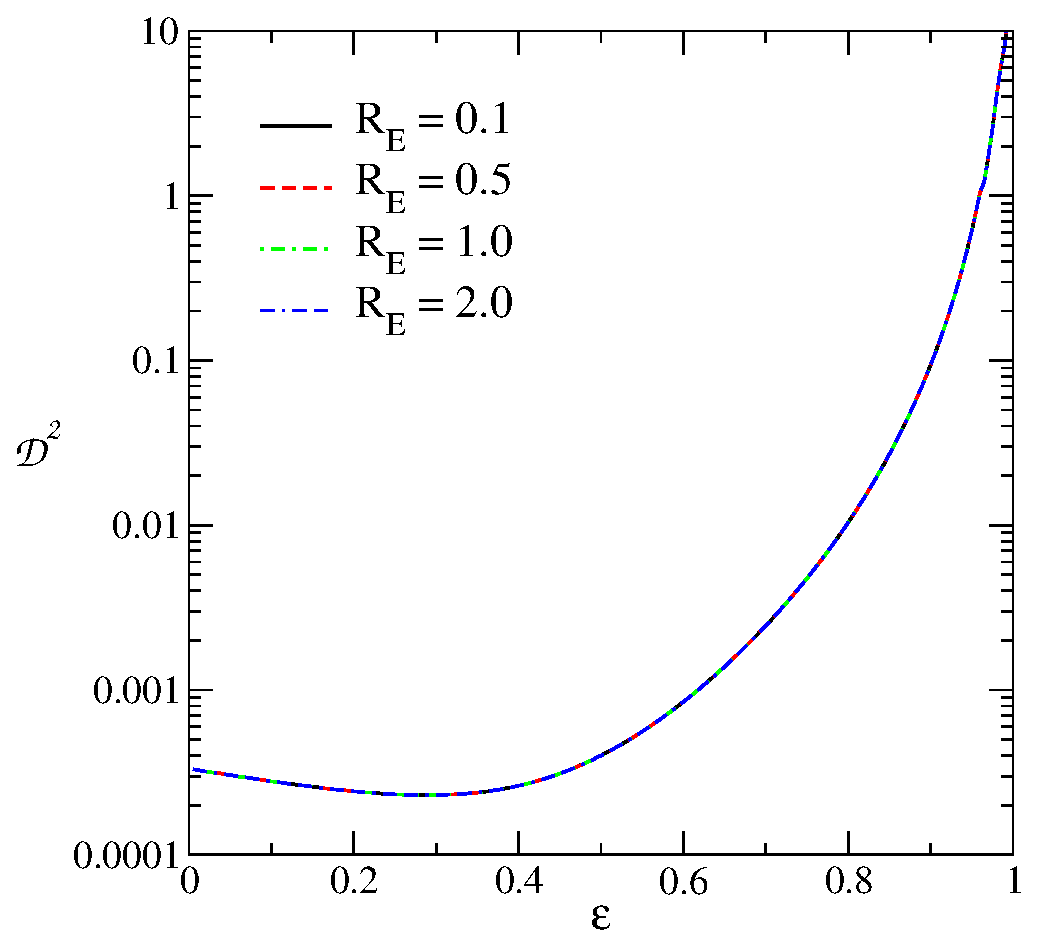
\includegraphics{d2_siep_caustic.eps}}
\caption{\label{d2_siep_plot} Mean weighted squared radial fractional difference
$\mathcal{D}^2$  as a function of ellipticity parameter for the tangential
caustic of the SIEP model.}
\end{center}
\end{figure}



\begin{figure*}
\begin{center}
\resizebox{\hsize}{!}{
\subfigure{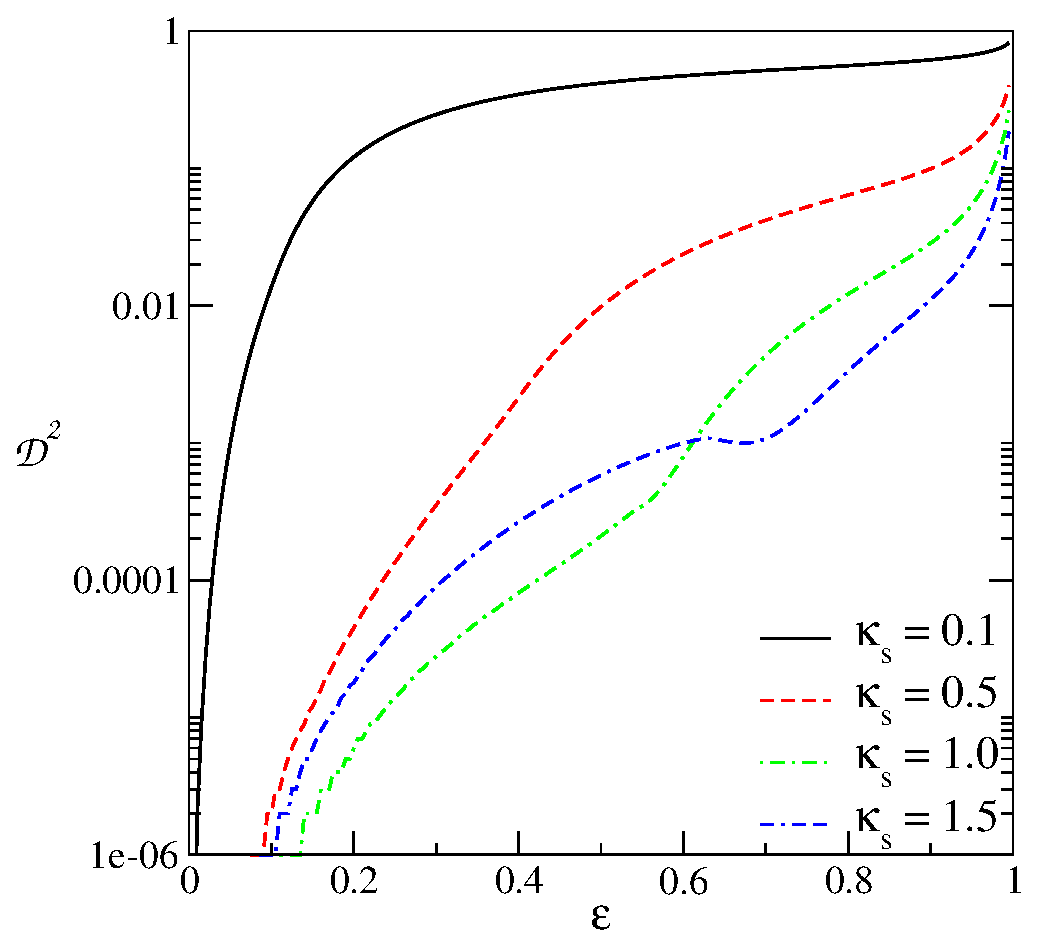
\includegraphics{d2_cc_pnfw.eps}} \hspace{1.5cm}
\subfigure{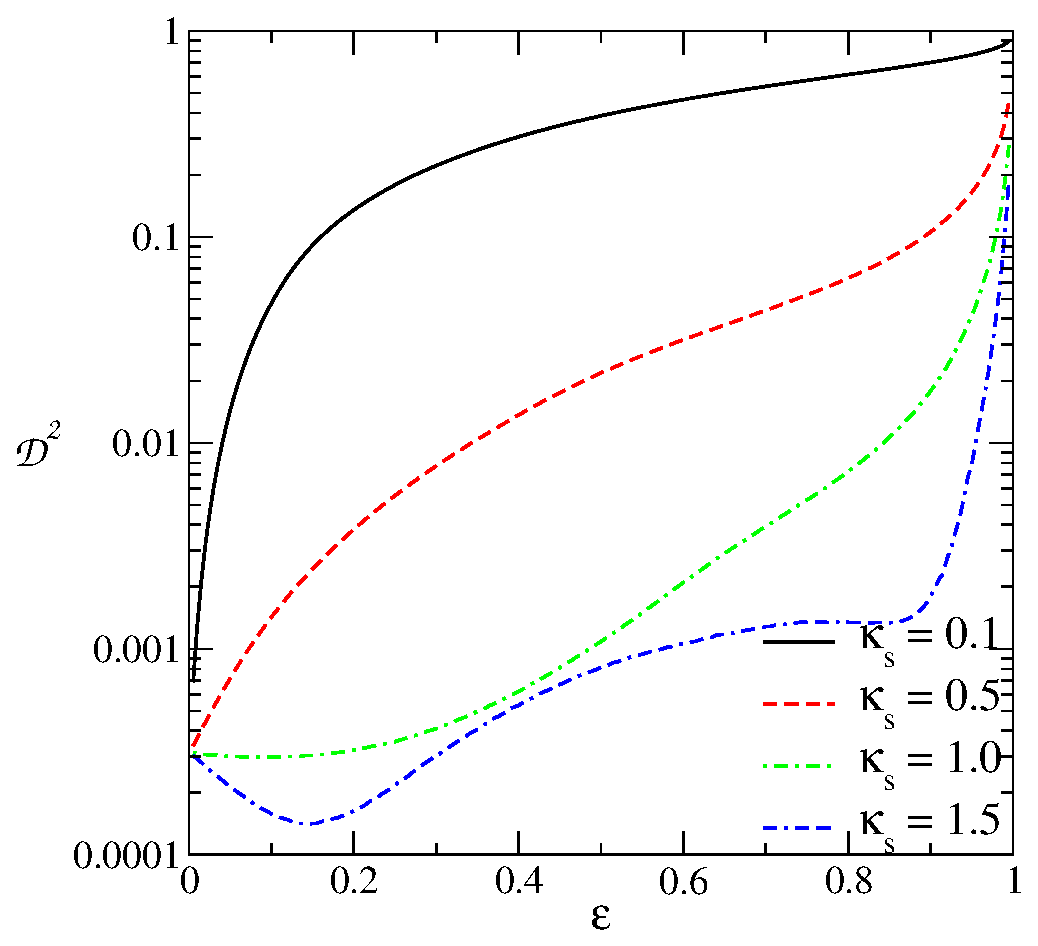
\includegraphics{d2_ca_pnfw.eps}}}
\caption{\label{d2_pnfw} Mean weighted squared radial fractional difference $\mathcal{D}^2$  as a function of ellipticity parameter for the PNFW model. Left Panel: For Critical Curves. Right Panel: For Caustics. Calculations where done for $r_s=1.0$}
\end{center}
\end{figure*}


\begin{itemize}
\item Introducing $\mathcal{D}^2$:

\begin{equation}
\mathcal{D}^ 2  :=\frac{\sum_{i=1}^N\,w_i[\tilde{r}_{\rm ES}(\theta_{i})-\tilde{r}_{\rm PA}(\theta_{i}) ]^2 }%
  {\sum_{i=1}^N w_i\, \tilde{r}_{\rm ES}^2(\theta_{i})},
  \label{D2_pm}
 \end{equation}
where $N$ is the number of data points, $\theta_i$ is the polar angle,
$w_i=\theta_i-\theta_{i-1}$ is a weight due the non uniform  distribution of points on $\phi$, $\tilde{r}_{\rm ES}(\theta_{i})$ and $\tilde{r}_{\rm PA}(\theta_{i})$ are the radial coordinate of tangential curves (both critic and caustic) of the exact solution and perturbative approach, respectively.


\begin{figure}
\begin{center}
\resizebox{\hsize}{!}{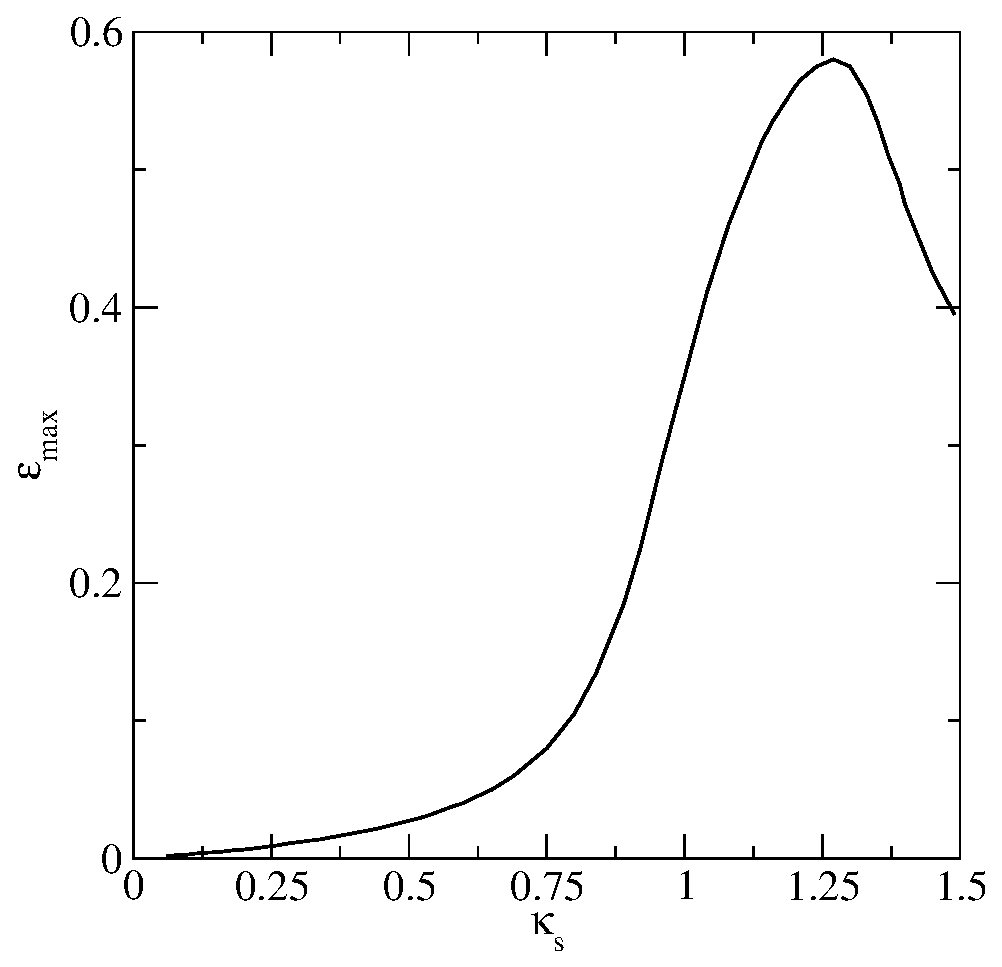
\includegraphics{cut_d2_caust.eps}}
\caption{\label{d2_cut_value} Maximum value of the ellipticity parameter such that the Perturbative Approach give an accurate calculation of critical curve and caustic. Here we use $\mathcal{D}^2=5\times 10^{-4}$ as cutoff value.}
\end{center}
\end{figure}



\item Discussion about Alard's Method to define the limits of validity:

The perturbative approach developed by Alard investigates small deviation from a circle of radius $R_{\rm E}$. This implies the gradient of the potential is linear near to $r=R_{\rm E}$ and the errors of this approximation is due to the deviation from the linearity. In particular, the gradient of the potential $\varphi_0$ must be close to the linear in the range in the image formation. Using equations (\ref{pot_expand}) and (\ref{fn-cn_def}), the condition of linearity is
\begin{equation}
D_{\rm max}=3|C_3|(r-R_{\rm E})_{\rm max}^2
\end{equation}
Now, we will derive a general expression for $C_3$ as a function of the lensing functions of axially-symmetric models. From equations (\ref{d2pot_circ}) and (\ref{kappa-gamma_circ})  is straightforward get to

\begin{equation}
C_3=2\left[\frac{d\kappa(r)}{dr}+\frac{\gamma(r)}{r}\right]_{r=R_{\rm E}}.
\end{equation}
For models coming from SIS, $C_3$ is null in everywhere. For models coming from NFW model it is possible to show that
\begin{equation}
C_3=\frac{4}{r^2_s-R^2_{\rm E}}\left[\frac{3}{2}R_{\rm E}\kappa(R_{\rm E})-\frac{\kappa_s\,r^2_s}{R_{\rm E}} \right]+2\frac{\gamma(R_{\rm E})}{R_{\rm E}}.
\end{equation}


\begin{figure}
\begin{center}
\resizebox{\hsize}{!}{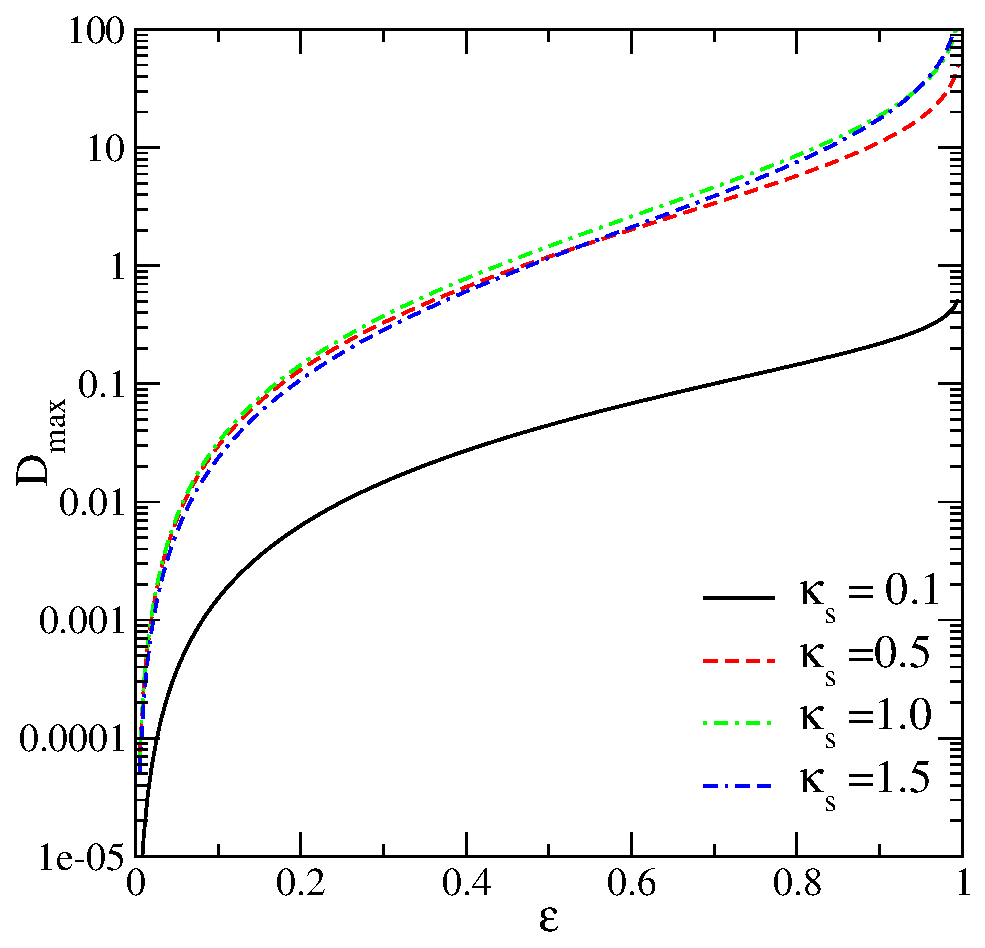
\includegraphics{dmax_e.eps}}
\caption{\label{dmax_plot} Alard's Method to quantify the limit of validity of the Perturbative Approach for the PNFW model. Calculations were done for $r_ s=1$. }
\end{center}
\end{figure}



\end{itemize}

\section{Local Deformation and Arc Cross Section}

\subsection{Local Deformation}

The Gravitational arc is commonly defined as a image for which its length-to-width ratio $L/W$ is above a given threshold
$(L/W)_{\rm th}$. Since the radial and tangential eigenvalues of the Jacobian matrix of the lens mapping, $\lambda_{+}$  and $\lambda_{-}$, describe well the properties of lensed images of infinitesimal circular sources, a good approximation for the length-to-width of arcs \citep{wu93,bartelmann94,haman97} is
\begin{equation}
\frac{L}{W}\simeq R_\lambda := \frac{\lambda_{2}}{\lambda_{1}}\label{lw}.
\end{equation}
 Note that, the approach given in Eq.~(\ref{lw}) replaces a measurement of a non-local quantity ($L/W$) by the calculation of a local quantity $\lambda_{2}/\lambda_{1}$. Despite such approximation is very useful for numerical computation of the arc properties, it takes into  account arcs generated through the highly distorted images of sources that do not cross the tangential caustic (the so-called deformation arcs), but not those from images of sources crossing the tangential caustic, the so-called merged arcs, \citep{rozo08,cunha10}.

 By following the Eq.~(\ref{lw}), tangential arcs with a given threshold $(L/W)_{\rm th} = R_{\rm th}$ are formed in the region limited  by the curves $R_\lambda=\pm R_{\rm th}$ (curves with constant distortion). The tangential critical curve ($\lambda_{-}=0$) will be given here by the condition $R_\lambda=\infty$. In most of this work we adopt the usual choice $R_{\rm th}=10$.

 \subsubsection{Local Deformation in the Exact Solution}

In General, the expression for the coordinates of the constant distortion curves are complicated to be obtain. For example, for the PNFW to solve the equation $R_\lambda=\pm R_{\rm th}$ is needed to use numerical method. While, for the SIEP model is possible to obtain an analytic solution.
From Eq.~(\ref{eigv_siep}) and (\ref{lw}) hence we have
\begin{equation}
R_{\rm th}=\frac{1}{1-\left[\mathcal{A}(\varepsilon)-\mathcal{B}(\varepsilon)\cos{2\theta_\varepsilon } \right](x_\varepsilon)^{-1}},
\end{equation}
and the pseudo-elliptical radial coordinates of the curves of constant distortion (in the lens plane) are
\begin{equation}
x_{\varepsilon,R_{\rm th}}=x_{\varepsilon,tcc}\times\left\{\begin{array}{cc} \frac{|R_{\rm th}|}{|R_{\rm th}|-1}, & R_{\rm th}>0 \\ & \\
\frac{|R_{\rm th}|}{|R_{\rm th}|+1}, & R_{\rm th}<0 \end{array}\right.
\end{equation}
The cartesian components of the constant distortion curves are given by Eqs.~(\ref{lens_eq_ad}) and (\ref{xtcc_cord}), for which $x_{\varepsilon,tcc}$ is replaced by $x_{\varepsilon,R_{\rm th}}$.

 \subsubsection{Local Deformation in the Perturbative Approach}
 In the case of the perturbative solution, for all kinds of model we can obtain an analytical solution for the constant distortion curves. From Eq.~(\ref{eigv_1-2_pa}) and (\ref{lw}) it is possible to show
\begin{equation}
r_{R_{\rm th}}=(x_{cc}+R_{\rm E})\times\left\{\begin{array}{cc} \frac{|R_{\rm th}|}{|R_{\rm th}|-1}, & R_{\rm th}>0 \\ & \\
\frac{|R_{\rm th}|}{|R_{\rm th}|+1}, & R_{\rm th}<0 \end{array}\right.
\end{equation}

\subsection{Cross Section for Deformation Arcs}

The efficiency of a lens to produce arcs with a given $(L/W)_{\rm th}$  is quantified by the cross section for arc formation (we will refer to it as the arc cross section). This arc cross section for deformation arcs is defined by the area in the source plane that satisfy $ L/W  \geq |R_{\rm th}|$ weighted by the multiplicity of the images, i.e
\begin{equation}
\sigma_{\rm dcs} \equiv \int d^2\eta =\int_{ R_\lambda > |R_{\rm th}|} \left |\rmn{det}\mathbfss{J}(\bmath{\xi}) \right| d^2\xi. \label{dcs_dim}
\end{equation}

\subsubsection{Cross Section for Deformation Arcs in the Exact Solution}
Here, we use a semi-analytic method to compute the arc cross section described in \citet{dm_2011}. In dimensionless coordinates $ \bmath{y}=\frac{\eta}{\eta_0}$ and $\bmath{x}=\frac{\xi}{\xi_0}$ we can write $\sigma_{\rm dcs}$ as
\begin{equation}
\sigma_{\rm dcs} = \xi_0^2\tilde{\sigma}_{\rm dcs}= \xi_0^2 \int_{ \frac{\lambda_r}{\lambda_t} > |R_{\rm th}|} \left |\rmn{det}\,\mathbfss{J}(\bmath{x}) \right| d^2\!x. \label{dcs_dimensionless}
\end{equation}

In general, the calculation of this expression requires numerical method, unless for a few kind of lens model.  For example, for the SIS model,
$\mathbfss{J}(\bmath{x})=1-\frac{1}{x}$, $\xi_0=R_{\rm E}$ and, hence we have

\begin{equation}
\sigma_{\rm SIS}=2\pi\,R^2_{\rm E} \frac{|R_{\rm th}|^2+1}{(|R_{\rm th}|^2-1)^2} \label{dcs_sis}
\end{equation}

The other  model that offers an analytical expression for the cross section for deformation arcs is the SIEP. For this model, the arc cross section for deformation arcs is

\begin{equation}
\sigma_{\rm SIEP}=R^2_{\rm E}\frac{|R_{\rm th}|^2+1}{(|R_{\rm th}|^2-1)^2}\frac{1}{\sqrt{a_{1\varepsilon} a_{2\varepsilon}}} (\sigma_1+\sigma_2
+\sigma_3)
\end{equation}
where
\begin{eqnarray*}
\sigma_1 &=& (0.75a^2_{1\varepsilon}+0.5 a_{1\varepsilon}a_{2\varepsilon}+0.75 a^2_{2\varepsilon})\arctan{\left(10^{8}\sqrt{\frac{a_{2\varepsilon}}{a_{1\varepsilon}}} \right)}\\
\sigma_2 &=& (a^2_{1\varepsilon}-a^ 2_{2\varepsilon})\sin{\left(2\arctan{\left( 10^{8}\sqrt{\frac{a_{2\varepsilon}}{a_{1\varepsilon}}}\right)}\right)} \\
\sigma_3&=& 0.0625(a_{1\varepsilon}-a_{2\varepsilon})^2\sin{\left(4\arctan{\left(10^{8}\sqrt{\frac{a_{2\varepsilon}}{a_{1\varepsilon}}} \right)}\right)}
\end{eqnarray*}
In the limit of $\varepsilon=0$, $\sigma_1=2\pi$, $\sigma_2=\sigma_3=0$, and we recover the Eq.~(\ref{dcs_sis}).

In the case of the PNFW, we use numerical method to integrate such area in the lens plane.



\subsubsection{Cross Section for Deformation Arcs in the Perturbative Approach}
Other advantage of the Perturbative Approach, is that allow obtain an analytical expression for the deformation cross section. Inserting Eq.~(\ref{eigv_1-2_pa}) in Eq.~(\ref{dcs_dim}) and by integrating in the radial coordinate is straightforward get to
\begin{equation}
\sigma_{dcs}=\kappa_2^2\frac{|R_{\rm th}|^2+1}{\left(|R_{\rm th}|^2-1\right)^2}\int_0^{2\pi}\left|\vec{
r}_{\mathrm{cc}}\right|^2\,{\rm d}\theta\label{sec-choq-pert-app2}
\end{equation}
For example, for the SIS model, for which $\kappa_2=1$ and $|\vec{r}_{cc}|=R_{\rm E}$, the analytical expression for the $\sigma$ is the same as Eq.~(\ref{dcs_sis}).

\subsection{Comparison between Cross Sections}

Aiming at quantifying the difference between both $\tilde{\sigma}_{\rm ES}$ and $\tilde{\sigma}_{\rm PA}$, we compute the relative difference
\begin{equation}
\frac{\Delta \tilde{\sigma}}{\tilde{\sigma}}=\left|\frac{\sigma_{\rm ES}-\sigma_{\rm PA}}{\sigma_{\rm ES}} \right|\label{dif_rela_sigma}.
\end{equation}


\begin{figure*}
\begin{center}
\resizebox{\hsize}{!}{
\subfigure{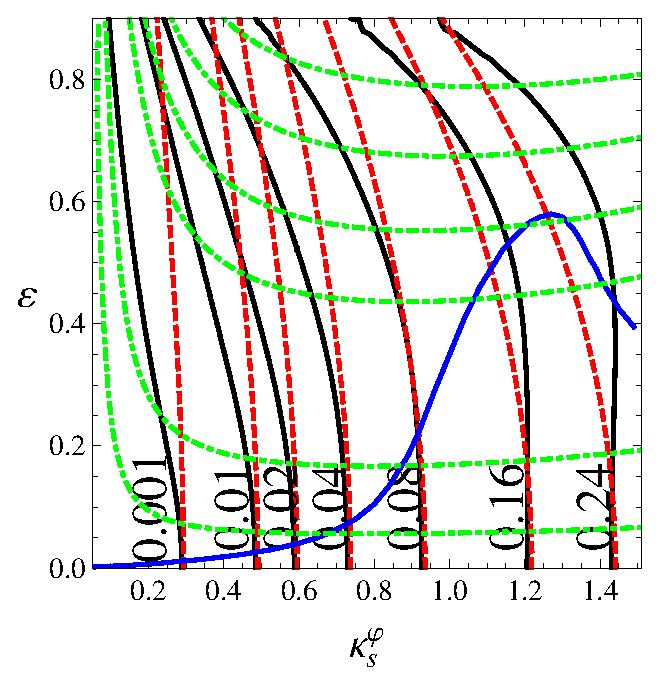
\includegraphics{fig7_pnfw_new.eps}} \hspace{1.5cm}
\subfigure{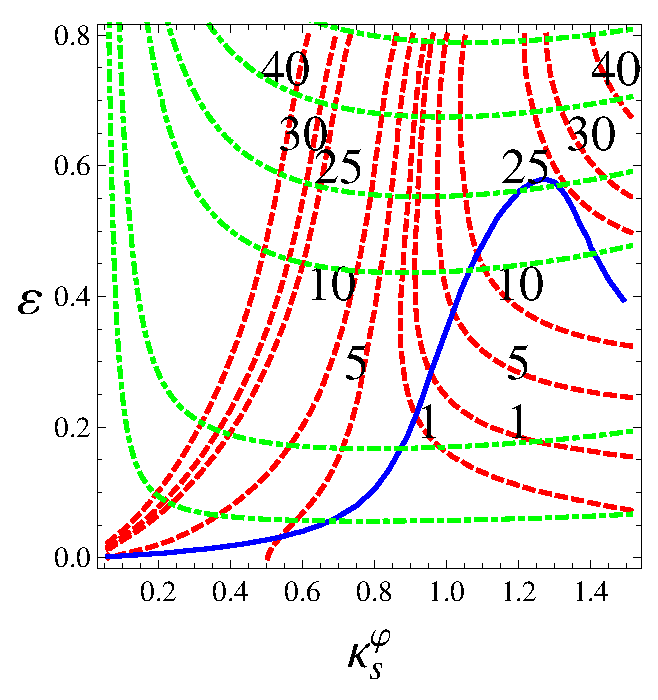
\includegraphics{drel_pnfw_new.eps}}}
\caption{\label{dcs_pnfw} Comparison between arc cross sections for the PNFW model. Left Panel: Contours of constant arc cross section in term of the PNFW parameters. Solid Lines correspond to Exact Solution and dashed lines correspond to Perturbative Approach.  Right Panel: Constant contours of  relative difference $\Delta\tilde{\sigma}/\tilde{\sigma}$(Eq.~\ref{dif_rela_sigma}) in \%. In both graphics, the blue solid line (later this curve will change by dotted line) shows $\varepsilon_{\rm max} (\kappa_s)$ line to guide the eyes and dot-dashed lines shows contour of $D_{\rm max}=0.01,0.1,1,2,4$ and $8$ (from bottom to the top). Calculation were done for $R_{\rm th}=10$. }
\end{center}
\end{figure*}



\begin{figure*}
\begin{center}
\resizebox{\hsize}{!}{
\subfigure{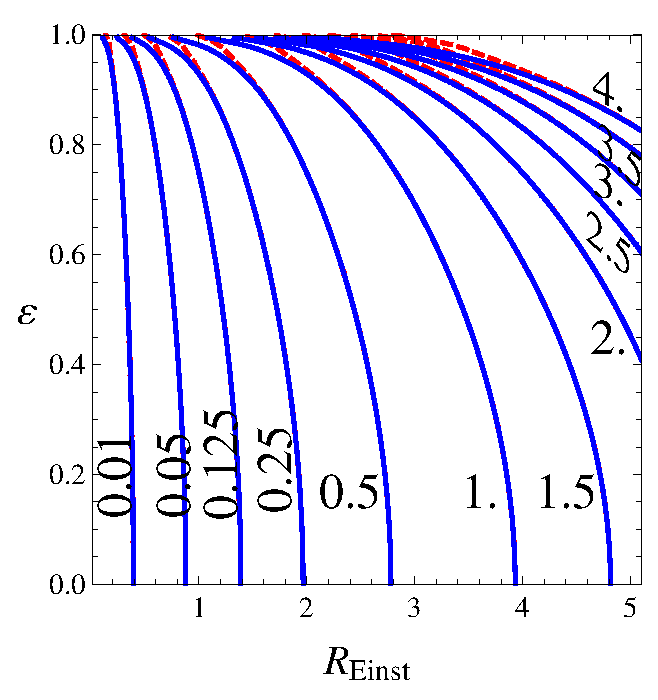
\includegraphics{fig_siep.eps}} \hspace{1.5cm}
\subfigure{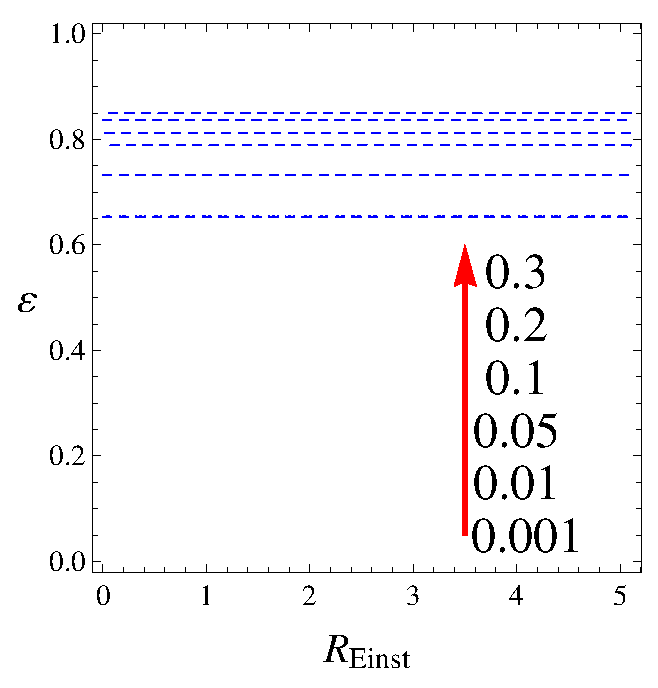
\includegraphics{drel_siep.eps}}}
\caption{\label{dcs_siep} Comparison between arc cross sections for the SIEP model. Left Panel: Contours of constant arc cross section in term of the SIEP parameters. Solid Lines correspond to the Exact Solution and dashed lines correspond to the Perturbative Approach.  Right Panel: Constant contours of  relative difference $\Delta\tilde{\sigma}/\tilde{\sigma}$ (Eq.~\ref{dif_rela_sigma}) in \%.}
\end{center}
\end{figure*}


\section{Concluding Remarks}


\section*{Acknowledgments}

We thank Marcos Lima for useful discussions.


\begin{thebibliography}{99}
%\bibitem[\protect\citeauthoryear{Author(s)}{Year}]{tag} Bibliography entry
%\bibitem[\protect\citeauthoryear{three_author_names}{first_author_etal}{Year}]{key} Bibliography entry
%
\bibitem[\protect\citeauthoryear{Alard}{2007}]{allard07} Alard,~C. 2007, MNRAS, 382, L58.
%
\bibitem[\protect\citeauthoryear{Alard}{2008}]{allard08} Alard,~C. 2008, MNRAS, 388, 375.
%
\bibitem[\protect\citeauthoryear{Bartelmann \& Weiss}{1994}]{bartelmann94} {Bartelmann},~M. \& {Weiss},~A. 1994, \aap, 287, 1


\bibitem[\protect\citeauthoryear{Bartelmann}{2003}]{bartelmann03} {Bartelmann},~M. 2003, astro-ph/0304162v1

\bibitem[\protect\citeauthoryear{Caminha et~al.}{2009}]{caminha09} {Caminha},~G.~B., {Estrada},~J., {Makler},~M., {et~al.} 2009, in preparation
%
\bibitem[\protect\citeauthoryear{D\'umet-Montoya, Caminha \& Makler}{D\'umet-Montoya et al.}{2011}]{dm_2011} D\'umet-Montoya,~H.~S., Caminha,~G.~B. and Makler,~M., 2011, A\&A submited, astro-ph/numero (DMCM).
%
\bibitem[\protect\citeauthoryear{Fedeli et~al.}{2006}]{fedeli05} {Fedeli},~C., {Meneghetti},~M., {Bartelmann},~M. {et~al.} 2006, \aap, 447, 419
%
\bibitem[\protect\citeauthoryear{Ferreira}{2010}]{cunha10} {Ferreira},~P. 2010, "Simulation and analysis of Gravitational Arcs", M.~D.~These, Federal University of Rio de Janeiro
%
\bibitem[\protect\citeauthoryear{Golse \& Kneib}{2002}]{gk02} Golse,~G., \& Kneib, ~J.-P. 2002, A\&A, 390, 821
%
\bibitem[\protect\citeauthoryear{Hamana \& Futamase}{1997}]{haman97} {Hamana},~T. \& {Futamase},~T. 1997, \mnras, 286, L7
%
\bibitem[\protect\citeauthoryear{Miralda-Escud\'e}{1991}]{miralda91} {Miralda-Escud\'e},~J. 1991, \apj, 370, 1
%
\bibitem[\protect\citeauthoryear{Navarro, Frenk \& White}{Navarro et~al.}{1996}]{nfw96} {Navarro},~J.~F., {Frenk},~C.~S., \& {White},~S.~D.~M. 1996, ApJ, 462, 563
%
\bibitem[\protect\citeauthoryear{Navarro, Frenk \& White}{Navarro et~al.}{1997}]{nfw97} {Navarro},~J.~F., {Frenk},~C.~S., \& {White},~S.~D.~M. 1997, ApJ, 490, 493

\bibitem [\protect\citeauthoryear{Schneider et~al.}{1992}]{SEF} {Schneider},~P., {Elhers},~J., \& {Falco}, ~E.~E. 1992, ``Gravitational lenses'', Springer-Verlag --Berlin

\bibitem[\protect\citeauthoryear{Rozo et~al.}{2008}]{rozo08} {Rozo},~E., {Nagai},~D., {Keeton},~C. {et~al.} 2008, \apj,  687, 22

\bibitem[\protect\citeauthoryear{Turnet et al.}{1984}]{turner84} Turner,~E.~L., Ostriker,~J.~P., \& Gott,~J.~R., 1984, \apj, 284,1

\bibitem[\protect\citeauthoryear{Wu \& Hammer}{1993}]{wu93} {Wu},~X.~P. \& {Hammer},~F. 1993, \mnras, 262, 187

\end{thebibliography}

\appendix

\section[]{\lowercase{Fitting function for} \mbox{{\boldmath $\varepsilon_{\rm max}$}} }

\label{lastpage}

\end{document}
%\begin{eqnarray}
%\kappa_\varepsilon(\bmath{x})&=&\mathcal{A}(\varepsilon)\kappa(x_\varepsilon)
%-\mathcal{B}(\varepsilon)\gamma(x_\varepsilon)\cos{2\theta_\varepsilon}
%\label{kappa_pnfw}\\
%\gamma_{1\varepsilon}(\bmath{x})& = &
%\mathcal{B}(\varepsilon)\kappa(x_\varepsilon)-\mathcal{A}
%(\varepsilon)\gamma(x_\varepsilon)\cos{2\theta_\varepsilon} \\
%\gamma_{2\varepsilon}(\bmath{x})& =
%&-\sqrt{\mathcal{A}^2(\varepsilon)-\mathcal{B}^2(\varepsilon)}
%\gamma(x_\varepsilon)\sin{ 2\theta_\varepsilon}\\
%\gamma^2_\varepsilon(\bmath{x}) & = &
%\mathcal{A}^2(\varepsilon)\gamma^2(x_\varepsilon)-2\mathcal{A}
%(\varepsilon)\mathcal {B}
%(\varepsilon)\kappa(x_\varepsilon)\gamma(x_\varepsilon)\cos{2\theta_\varepsilon}
%\nonumber  \\ &  &
%+\mathcal{B}^2(\varepsilon)[\kappa^2(x_\varepsilon)-\sin^2{2\theta_\varepsilon}
%\gamma^2(x_\varepsilon) ]\label{gamma_pnfw}
%\end{eqnarray}
